\section{Model}
\label{sec:model}

\subsection{Network Representation}

We model each dataset as a directed graph $G = (V, E)$ where $V$ is the
set of nodes (users or email addresses) and $E \subseteq V \times V$ is the
set of directed edges (interactions).
For the Facebook dataset we use an undirected graph $G = (V, E)$ since
friendship is a symmetric relation.
Edge weights, where present, encode interaction frequency (e.g.\ number
of retweets between a pair of users).

\subsection{Centrality Metrics}

We compute four node-level centrality measures.

\textbf{In-degree centrality.}
For a node $v$, $k^{\text{in}}(v) = |\{u : (u,v) \in E\}|$ counts the number
of incoming edges. In interaction networks, high in-degree corresponds to
nodes that are frequently targeted (e.g.\ popular accounts).

\textbf{Out-degree centrality.}
$k^{\text{out}}(v) = |\{u : (v,u) \in E\}|$ counts outgoing edges and
identifies prolific senders or broadcasters.

\textbf{Betweenness centrality.}
\begin{equation}
    C_B(v) = \sum_{s \neq v \neq t} \frac{\sigma_{st}(v)}{\sigma_{st}}
\end{equation}
where $\sigma_{st}$ is the total number of shortest paths from $s$ to $t$
and $\sigma_{st}(v)$ is the number of those paths that pass through $v$.
Nodes with high betweenness act as \textit{bridges} connecting otherwise
distant parts of the network.

\textbf{Eigenvector centrality.}
The eigenvector centrality vector $\mathbf{x}$ satisfies
$A\mathbf{x} = \lambda_{\max} \mathbf{x}$,
where $A$ is the adjacency matrix and $\lambda_{\max}$ is the largest
eigenvalue. High eigenvector centrality identifies nodes that are connected
to other important nodes, capturing recursive influence.

\subsection{Community Detection}

We apply the \textit{Louvain algorithm} \citep{blondel2008} to detect
communities by iteratively maximizing modularity
\begin{equation}
    Q = \frac{1}{2m} \sum_{ij} \left[ A_{ij} - \frac{k_i k_j}{2m} \right]
        \delta(c_i, c_j),
\end{equation}
where $m = |E|$, $k_i$ is the degree of node $i$, and $\delta(c_i, c_j) = 1$
iff nodes $i$ and $j$ are in the same community.
For directed networks (Higgs, Enron) we convert to an undirected graph
prior to community detection.

\subsection{Graph-Level Properties}

Beyond node-level centrality, we measure two graph-level structural
properties~\citep{newman2018networks}.

\textbf{Clustering coefficient.}
The local clustering coefficient of node $v$ is
\begin{equation}
    c(v) = \frac{|\{(u,w) \in E : u,w \in \mathcal{N}(v)\}|}{k(v)(k(v)-1)},
\end{equation}
where $\mathcal{N}(v)$ is the set of neighbours of $v$ and $k(v) = |\mathcal{N}(v)|$.
The network average $\bar{C} = \frac{1}{|V|}\sum_v c(v)$ quantifies the
tendency of nodes to form tightly connected triples.
High $\bar{C}$ relative to a random graph is a hallmark of
small-world networks~\citep{watts1998}.

\textbf{Average shortest-path length.}
\begin{equation}
    \ell = \frac{1}{|V|(|V|-1)} \sum_{s \neq t} d(s,t),
\end{equation}
where $d(s,t)$ is the length of the shortest path from $s$ to $t$.
For large networks we estimate $\ell$ via BFS sampling from
500 randomly chosen source nodes in the largest connected component.

\subsection{Top-10\% Intersection Analysis}

To assess agreement between metrics, we compute the pairwise intersection
of nodes appearing in the top 10\% of each centrality ranking.
A large intersection between, say, betweenness and in-degree indicates
that popular nodes also serve as structural bridges;
a small intersection indicates that hubs and bridges are structurally
distinct populations.

\begin{figure*}[ht]
    \centering
    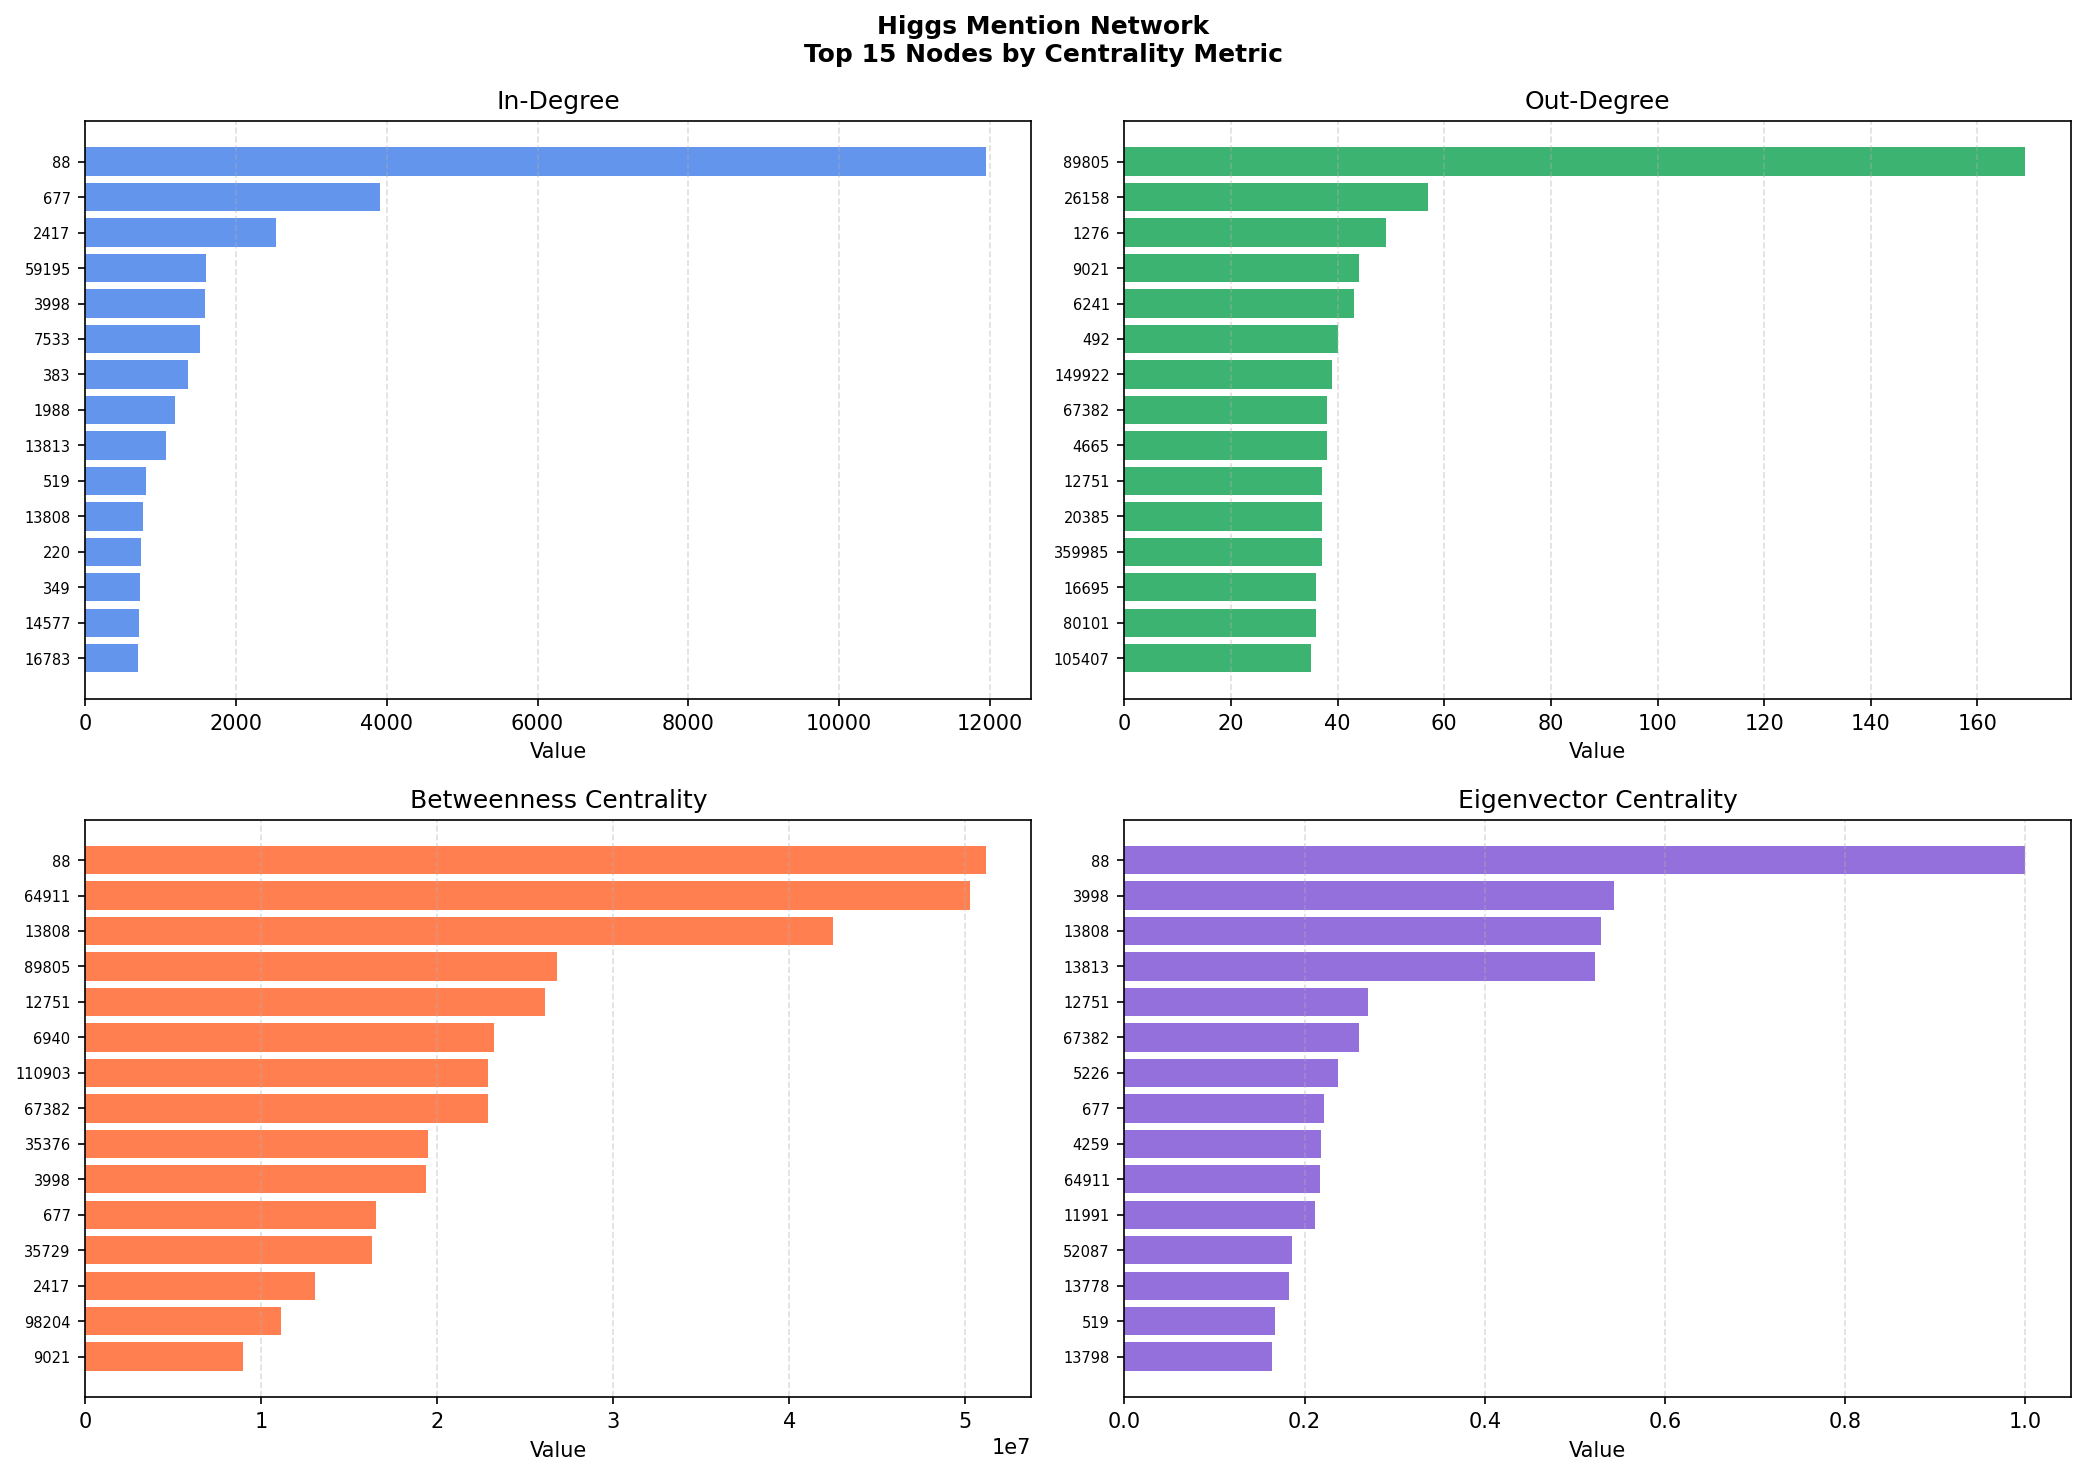
\includegraphics[width=0.95\linewidth]{figures/higgs_mention_centrality.png}
    \caption{Top-15 nodes by each centrality metric in the Higgs Mention network.
             Node \texttt{88} dominates in-degree and eigenvector centrality while
             node \texttt{64911} ranks highest in betweenness, illustrating the
             hub--bridge distinction described in Section~\ref{sec:model}.}
    \label{fig:mention_centrality}
\end{figure*}
